\section{Evaluation}
\label{sec:eval}

We ask four questions. How much faster is \cape{} than fixed windows, synchronous decoding and AdaEDL, and at what energy cost (Section~\ref{sec:main})? Where do its gains come from (Section~\ref{sec:why})? Do the results hold across tasks, prompts and evaluation sets (Section~\ref{sec:robust})? And how do exactness, task accuracy and overhead behave (Section~\ref{sec:integrity})?

\subsection{Methodology}
\emph{Workloads.} Prompts come from our local subsets of GSM8K~\cite{gsm8k2021} (50 grade-school math problems), HumanEval~\cite{humaneval2021} (30 Python function completions) and the first-turn questions of MT-Bench~\cite{mtbench2023} (30 open-ended writing and reasoning prompts). Generation uses the Llama~3 chat template, greedy decoding and at most 512 output tokens. Every request runs once with 2\,ms and once with 100\,ms of added delay per verification.

\emph{Evaluation sets.} The main evaluation runs all seven methods below on all \E{full:prompts} prompts at both delays, \E{full:requests:fmt} measured requests in total. Before it, \cape{}'s default setting was evaluated on two held-out sets of \E{h1:prompts} and \E{h2:prompts} prompts (\E{h1:requests} requests each), against Fixed-4, a heuristic latency-regime controller and a variant with more elaborate estimators. Neither the held-out sets nor the main evaluation were used to design or tune \cape{}. The held-out sets ran with the draft server configured with four slots and an 8,192-token context; single-stream draft speed was unchanged.

\emph{Protocol.} For each evaluation, the methods, prompts, seeds, delays and analysis were frozen in a plan file before the first measured request. Methods are interleaved in a randomized, balanced order within each prompt--delay block. Reference outputs and equal 16-token warm-ups are generated before timing starts, and no request is retried. The main evaluation was interrupted once by a dropped connection to the cloud server and resumed with the same plan; the interrupted request was run again. Throughput is the total number of output tokens divided by the total wall time, including terminal lookahead. Energy per token is the integrated board energy divided by the number of output tokens. Paired effects come with 95\% percentile intervals from 2,000 bootstrap resamples of prompts. A positive J/token saving means less energy per token.

\emph{Methods.} All methods share the models, servers, token-ID transport and strict greedy verification.
\begin{itemize}
\item \textbf{Sync-4}: synchronous speculative decoding with four draft tokens per round and no lookahead.
\item \textbf{Fixed-$\gamma$}, $\gamma\in\{2,4,8\}$: $\gamma$ draft tokens per round with a complete-block lookahead of $h=\gamma+1$. Fixed-4 is the fastest fixed window pooled over both delays and the reference for all relative numbers.
\item \textbf{AdaEDL}~\cite{adaedl2024}: synchronous decoding that streams up to eight draft tokens and stops before the first token whose entropy-based acceptance bound $1-\sqrt{0.2\,H}$ falls below an adaptive threshold. We use the paper's update rule and hyper-parameters. The entropy is computed from the top-20 draft probabilities plus the residual mass. The initial threshold, which the paper does not specify, is set to 0.5, the best of five values on development prompts.
\item \textbf{\cape{}} with $w=0$ (\capes{}, speed), $w=0.25$ (\cape{}, default; held-out sets) and $w=0.5$ (\capee{}, energy).
\item \textbf{Regime} (held-out Set~1 only): a latency-regime heuristic from our earlier work. After a four-token warm-up, it chooses among complete-block windows $\gamma\in\{2,4,6,8\}$ from the measured verification interval and admits longer windows only when the measured overlap allows them.
\end{itemize}

\begin{table*}[t]
\centering
\caption{Main evaluation: \E{full:prompts} prompts, two delays, \E{full:requests:fmt} requests. Throughput and J/token per method; paired effects relative to Fixed-4 with 95\% prompt-cluster bootstrap intervals; draft-server busy time per output token and discarded draft tokens per 100 output tokens.}
\label{tab:main}
\footnotesize
\setlength{\tabcolsep}{3.5pt}
\begin{tabular}{@{}lrrrrllrr@{}}
\toprule
 & \multicolumn{3}{c}{Throughput (tok/s)} & J/token & \multicolumn{2}{c}{Relative to Fixed-4, 2 and 100\,ms pooled} & Draft busy & Discarded\\
\cmidrule(lr){2-4}\cmidrule(lr){6-7}
Method & 2\,ms & 100\,ms & pooled & pooled & Throughput gain (\%) & J/token saving (\%) & ms/token & per 100 tok.\\
\midrule
Sync-4 & 13.86 & 9.74 & 11.43 & 0.650 & $-23.4$ [$-$24.9, $-$21.9] & $+13.1$ [11.1, 15.0] & 35.9 & 0 \\
Fixed-2 & 15.94 & 9.78 & 12.11 & 0.708 & $-18.8$ [$-$20.7, $-$16.8] & $+5.4$ [3.4, 7.4] & 43.0 & 40 \\
Fixed-4 & 18.07 & 12.71 & 14.92 & 0.748 & \multicolumn{2}{c}{baseline} & 48.3 & 67 \\
Fixed-8 & 14.54 & 13.41 & 13.95 & 0.979 & $-6.5$ [$-$9.4, $-$3.4] & $-30.9$ [$-$34.2, $-$27.4] & 73.1 & 120 \\
AdaEDL & 13.30 & 9.83 & 11.30 & 0.731 & $-24.3$ [$-$25.2, $-$23.3] & $+2.3$ [1.2, 3.3] & 44.7 & 0 \\
\textbf{CAPE-S} & 19.19 & 14.30 & 16.40 & 0.772 & $+9.9$ [8.0, 12.0] & $-3.2$ [$-$4.8, $-$1.6] & 52.1 & 89 \\
\textbf{CAPE-E} & 18.42 & 12.68 & 15.02 & 0.703 & $+0.7$ [$-$1.3, 3.1] & $+6.1$ [4.5, 7.7] & 44.4 & 55 \\
\bottomrule
\end{tabular}

\end{table*}

\begin{figure*}[t]
\centering
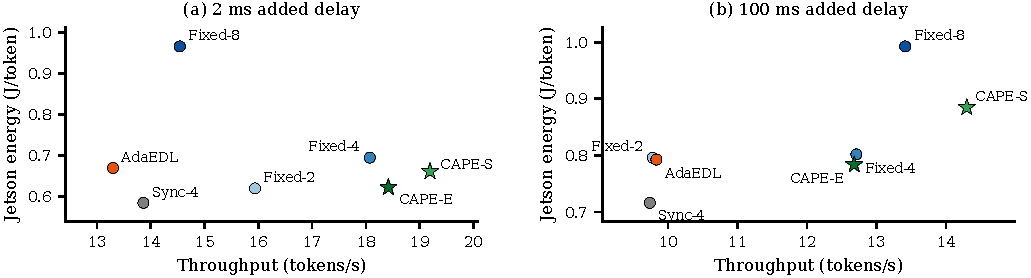
\includegraphics[width=0.92\textwidth]{figures/tradeoff.pdf}
\caption{Speed and energy of all methods in the main evaluation; points further right and lower are better. \capes{} is the fastest method at both delays. \capee{} is about as frugal as Fixed-2 at 2\,ms while much faster, and has the lowest J/token of all lookahead methods at 100\,ms.}
\label{fig:tradeoff}
\end{figure*}

\subsection{Main results}
\label{sec:main}
Table~\ref{tab:main} and Fig.~\ref{fig:tradeoff} summarize the main evaluation; Fig.~\ref{fig:effects} shows the paired effects with their intervals.

\emph{Lookahead is essential across a network, but no fixed window fits all delays.} Fixed-4 is \E{full:fixed4:sync4:pooled:abssp} \E{full:fixed4:sync4:pooled:spci} faster than Sync-4, at the price of \E{full:fixed4:sync4:pooled:abssv} more J/token. Fixed-4 is the fastest fixed window at 2\,ms. At 100\,ms, Fixed-8 is \E{full:fixed8:fixed4:high:abssp} faster than Fixed-4, but it uses \E{full:fixed8:fixed4:high:abssv} more energy per token there and is \E{full:fixed8:fixed4:low:abssp} slower at 2\,ms. Fixed-2 emits too few tokens per round and is \E{full:fixed2:fixed4:pooled:abssp} slower than Fixed-4 overall.

\emph{Adapting the draft length alone does not help here.} AdaEDL stops drafting when acceptance becomes unlikely, which saves target computation when verification cost grows with the draft. In the edge--cloud setting, verification cost is nearly independent of the draft length (Observation~2), and the device idles during every round trip. AdaEDL is therefore not faster than Sync-4 (\E{full:adaedl:sync4:pooled:sp} \E{full:adaedl:sync4:pooled:spci}) and uses \E{full:adaedl:sync4:pooled:abssv} more J/token, because it drafts longer blocks and streams draft probabilities.

\emph{\capes{} is the fastest method.} \capes{} raises throughput by \E{full:capes:fixed4:pooled:abssp} \E{full:capes:fixed4:pooled:spci} over Fixed-4. At 2\,ms it is \E{full:capes:fixed4:low:abssp} \E{full:capes:fixed4:low:spci} faster \emph{and} uses \E{full:capes:fixed4:low:abssv} \E{full:capes:fixed4:low:svci} less energy per token. At 100\,ms it is \E{full:capes:fixed4:high:abssp} \E{full:capes:fixed4:high:spci} faster, buying speed with \E{full:capes:fixed4:high:abssv} more J/token; over both delays its J/token is \E{full:capes:fixed4:pooled:abssv} higher. \capes{} also beats an oracle that picks the best fixed window for each delay. It is \E{full:capes:fixed4:low:abssp} faster than Fixed-4 at 2\,ms and \E{full:capes:fixed8:high:abssp} \E{full:capes:fixed8:high:spci} faster than Fixed-8 at 100\,ms, where it also uses \E{full:capes:fixed8:high:abssv} less energy per token. It is \E{full:capes:sync4:pooled:abssp} faster than Sync-4 and \E{full:capes:adaedl:pooled:abssp} faster than AdaEDL.

\emph{\capee{} saves energy at the speed of the fastest fixed window.} \capee{} matches Fixed-4's throughput (\E{full:capee:fixed4:pooled:sp} \E{full:capee:fixed4:pooled:spci}) and lowers J/token by \E{full:capee:fixed4:pooled:abssv} \E{full:capee:fixed4:pooled:svci}, by \E{full:capee:fixed4:low:abssv} at 2\,ms. It dominates AdaEDL (\E{full:capee:adaedl:pooled:sp} throughput, \E{full:capee:adaedl:pooled:sv} J/token saving) and Fixed-8 (\E{full:capee:fixed8:pooled:sp} and \E{full:capee:fixed8:pooled:sv}), with all four intervals excluding zero. It is \E{full:capee:fixed2:pooled:abssp} faster than Fixed-2 at equal energy (\E{full:capee:fixed2:pooled:sv} \E{full:capee:fixed2:pooled:svci}). Compared with Sync-4, the most frugal method, \capee{} is \E{full:capee:sync4:pooled:abssp} faster for \E{full:capee:sync4:pooled:abssv} more J/token.

\emph{One weight selects the operating point.} Raising $w$ from 0 to 0.5 trades \E{full:capee:capes:pooled:abssp} of throughput for \E{full:capee:capes:pooled:abssv} lower J/token. Both settings lie on the speed--energy frontier of Fig.~\ref{fig:tradeoff}: no other method is both faster and more frugal than either of them at either delay.

\begin{figure}[t]
\centering
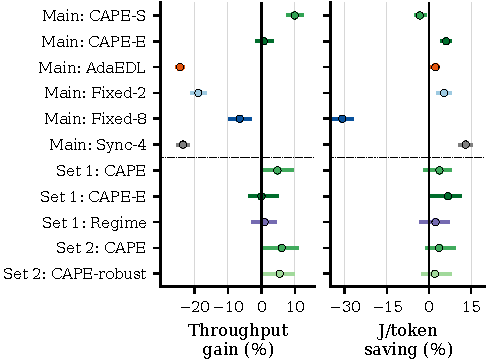
\includegraphics[width=\columnwidth]{figures/effects.pdf}
\caption{Paired effects relative to Fixed-4 (2 and 100\,ms pooled) with 95\% prompt-cluster bootstrap intervals. Above the dotted line: main evaluation (\E{full:prompts} prompts); below: held-out sets.}
\label{fig:effects}
\end{figure}

\begin{figure}[t]
\centering
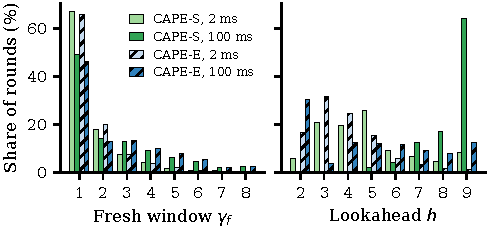
\includegraphics[width=\columnwidth]{figures/controller.pdf}
\caption{Fresh windows and lookahead lengths chosen by \capes{} and \capee{} in the main evaluation. Fresh windows stay short; lookahead grows with delay, and less so when energy is weighted.}
\label{fig:controller}
\end{figure}

\subsection{Where the gains come from}
\label{sec:why}
Fig.~\ref{fig:controller} shows the decisions behind these results. \cape{} keeps the critical path short: the mean fresh window of \capes{} is \E{ctl:full:capes:low:fresh} tokens at 2\,ms and \E{ctl:full:capes:high:fresh} at 100\,ms, against four for Fixed-4. It sizes the lookahead to the round trip: the mean lookahead of \capes{} grows from \E{ctl:full:capes:low:h} to \E{ctl:full:capes:high:h} tokens when the delay increases. \capee{} prices speculative work and grows its lookahead only from \E{ctl:full:capee:low:h} to \E{ctl:full:capee:high:h} tokens. This behavior emerges from Eq.~\eqref{eq:objective} and the online estimates; no delay threshold is configured.

The lookahead is also better used. \capes{} and \capee{} reuse \E{reuse:capes} and \E{reuse:capee} of their lookahead blocks, against \E{reuse:fixed4} for Fixed-4. \capee{} discards \E{full:capee:pooled:waste} draft tokens per 100 output tokens, against \E{full:fixed4:pooled:waste} for Fixed-4, and keeps the draft server busy for \E{full:capee:pooled:busy}\,ms per output token instead of \E{full:fixed4:pooled:busy}\,ms, which explains its energy saving through Eq.~\eqref{eq:energy}. \capes{} spends more draft time (\E{full:capes:pooled:busy}\,ms per token) to buy speed, as instructed by $w=0$.

\begin{table*}[t]
\centering
\caption{Effects of \capes{} and \capee{} relative to Fixed-4 by task (both delays pooled) and by delay (all tasks pooled), with 95\% prompt-cluster bootstrap intervals.}
\label{tab:breakdown}
\footnotesize
\setlength{\tabcolsep}{4pt}
\begin{tabular}{@{}llccccc@{}}
\toprule
Method & Effect (\%) & GSM8K & HumanEval & MT-Bench & 2\,ms & 100\,ms\\
\midrule
CAPE-S & throughput gain & $+8.9$ [5.6, 12.1] & $+17.8$ [14.7, 21.3] & $+5.7$ [4.2, 7.6] & $+6.2$ [3.6, 8.9] & $+12.5$ [10.2, 14.9] \\
CAPE-S & J/token saving & $-1.7$ [$-$3.9, 0.7] & $-0.4$ [$-$2.4, 1.6] & $-6.5$ [$-$8.9, $-$3.8] & $+4.9$ [2.9, 7.0] & $-10.4$ [$-$12.3, $-$8.3] \\
CAPE-E & throughput gain & $-0.3$ [$-$2.6, 2.4] & $+11.5$ [7.8, 16.1] & $-5.0$ [$-$6.4, $-$3.2] & $+1.9$ [$-$0.4, 4.9] & $-0.3$ [$-$2.7, 2.5] \\
CAPE-E & J/token saving & $+4.3$ [2.6, 6.2] & $+0.6$ [$-$1.1, 2.5] & $+11.7$ [9.1, 14.6] & $+10.5$ [8.4, 12.5] & $+2.3$ [0.9, 3.6] \\
\bottomrule
\end{tabular}

\end{table*}

\subsection{Robustness across tasks, prompts and sets}
\label{sec:robust}
\emph{Tasks.} Table~\ref{tab:breakdown} breaks the effects down by task. \capes{} is faster than Fixed-4 on every task: by \E{full:capes:fixed4:gsm8k:abssp} on GSM8K, \E{full:capes:fixed4:humaneval:abssp} on HumanEval and \E{full:capes:fixed4:mtbench:abssp} on MT-Bench, with all intervals above zero. MT-Bench has the lowest acceptance rate (\E{acc:full:mtbench} with Fixed-4, against \E{acc:full:gsm8k} for GSM8K and \E{acc:full:humaneval} for HumanEval). There, \capes{} pays for its speed with \E{full:capes:fixed4:mtbench:abssv} more J/token, whereas \capee{} saves \E{full:capee:fixed4:mtbench:abssv} at \E{full:capee:fixed4:mtbench:abssp} lower throughput because it stops prefetching blocks that are unlikely to be used. On HumanEval, \capee{} is also \E{full:capee:fixed4:humaneval:abssp} faster than Fixed-4 at unchanged energy.

\emph{Prompts and host activity.} Some of the \E{full:prompts} prompts had appeared in earlier recorded phases (the held-out sets, a pilot comparison and the AdaEDL threshold sweep). On the \E{rob:fresh} prompts outside these phases, \capes{} gains \E{rob:fresh:capes:abssp} \E{rob:fresh:capes:spci} in throughput and \capee{} saves \E{rob:fresh:capee:abssv} \E{rob:fresh:capee:svci} of J/token. While the main evaluation ran, we briefly used the host for analysis and logged each period. Excluding the \E{rob:blocks} prompt--delay blocks that overlap these periods leaves the results unchanged (\E{rob:clean:capes:abssp} faster and \E{rob:clean:capee:abssv} less J/token).

\begin{table}[t]
\centering
\caption{Held-out sets with \cape{}'s default setting ($w=0.25$), 2 and 100\,ms pooled. Gains are relative to Fixed-4 with 95\% prompt-cluster bootstrap intervals.}
\label{tab:heldout}
\footnotesize
\setlength{\tabcolsep}{2.4pt}
\begin{tabular}{@{}lrrll@{}}
\toprule
Method & tok/s & J/tok & Throughput gain (\%) & J/token saving (\%)\\
\midrule
\multicolumn{5}{@{}l}{\emph{Set 1: 9 prompts, 72 requests}} \\
Fixed-4 & 13.44 & 0.849 & \multicolumn{2}{c}{baseline} \\
Regime & 13.57 & 0.829 & $+0.9$ [$-$2.4, 4.1] & $+2.4$ [$-$2.9, 6.7] \\
CAPE & 14.09 & 0.817 & $+4.8$ [1.2, 9.3] & $+3.7$ [$-$1.5, 7.6] \\
CAPE-E & 13.44 & 0.791 & $+0.0$ [$-$3.4, 4.5] & $+6.8$ [0.2, 11.2] \\
\midrule
\multicolumn{5}{@{}l}{\emph{Set 2: 12 prompts, 72 requests}} \\
Fixed-4 & 14.87 & 0.788 & \multicolumn{2}{c}{baseline} \\
CAPE & 15.77 & 0.760 & $+6.0$ [1.1, 10.7] & $+3.6$ [$-$0.6, 9.0] \\
CAPE-robust & 15.68 & 0.772 & $+5.4$ [0.4, 9.5] & $+2.1$ [$-$2.2, 7.4] \\
\bottomrule
\end{tabular}

\end{table}

\emph{Held-out sets.} Table~\ref{tab:heldout} shows the two held-out sets, which were run before the main evaluation. The default setting ($w=0.25$) increased throughput over Fixed-4 by \E{h1:cape:fixed4:pooled:abssp} \E{h1:cape:fixed4:pooled:spci} and \E{h2:cape:fixed4:pooled:abssp} \E{h2:cape:fixed4:pooled:spci} without a measurable energy penalty (J/token savings of \E{h1:cape:fixed4:pooled:sv} and \E{h2:cape:fixed4:pooled:sv}). It was \E{h1:cape:regime:pooled:abssp} \E{h1:cape:regime:pooled:spci} faster than the Regime heuristic, whose own gain over Fixed-4 was \E{h1:regime:fixed4:pooled:sp} \E{h1:regime:fixed4:pooled:spci}. A variant with more elaborate estimators (hierarchical shrinkage of acceptance, an expected-maximum round-trip estimate and a restricted action set) changed throughput by \E{h2:caperobust:cape:pooled:sp} \E{h2:caperobust:cape:pooled:spci} relative to \cape{}, so the simple estimators of Section~\ref{sec:design} suffice.

\begin{table}[t]
\centering
\caption{Outputs in the main evaluation (220 requests per method): GSM8K answers correct out of 100, truncations at 512 tokens, request pairs whose token sequence differs from Fixed-4 ($\neq$), and outputs identical to the cloud's own autoregressive generation ($=$ cloud AR).}
\label{tab:quality}
\footnotesize
\setlength{\tabcolsep}{2.6pt}
\begin{tabular}{@{}lcccc@{}}
\toprule
Method & GSM8K & Truncated & $\neq$ Fixed-4 & $=$ cloud AR\\
\midrule
Sync-4 & 72/100 & 23/220 & 1 & 83/220 \\
Fixed-2 & 72/100 & 24/220 & 20 & 85/220 \\
Fixed-4 & 72/100 & 23/220 & --- & 83/220 \\
Fixed-8 & 74/100 & 17/220 & 26 & 84/220 \\
AdaEDL & 74/100 & 19/220 & 14 & 84/220 \\
CAPE-S & 73/100 & 23/220 & 19 & 86/220 \\
CAPE-E & 73/100 & 24/220 & 19 & 84/220 \\
\bottomrule
\end{tabular}

\end{table}

\subsection{Exactness, task accuracy and overhead}
\label{sec:integrity}
All \E{full:requests:fmt} requests completed with valid power traces. Every emitted token is the target's top choice under the verification pass, yet outputs are not always identical across methods (Table~\ref{tab:quality}). In \E{ident:full:differing} of the \E{ident:full:blocks} prompt--delay blocks, at least one method's output differs from the others, typically after many identical tokens (median first difference at token \E{div:median} between Fixed-4 and \capes{}). The differences track the size of the verified window rather than the controller. Sync-4, which verifies the same four-token windows as Fixed-4, differs from it in only \E{full:sync4:fixed4:pooled:chg} of 220 requests. Fixed windows of other sizes differ as often as \cape{} (Fixed-2: \E{full:fixed2:fixed4:pooled:chg}, Fixed-8: \E{full:fixed8:fixed4:pooled:chg}, \capes{}: \E{full:capes:fixed4:pooled:chg}). This is consistent with near-tied scores of the quantized target that resolve differently for different numbers of verified positions. The same sensitivity separates speculative decoding from the cloud's own autoregressive generation: every method, including Fixed-4, reproduces it exactly in only \E{q:ref:min}--\E{q:ref:max} of 220 requests.

These differences do not affect task accuracy. GSM8K accuracy ranges from \E{q:gsm8k:min} to \E{q:gsm8k:max} correct answers out of 100 across all methods (Fixed-4: \E{q:fixed4:gsm8k}, \capes{}: \E{q:capes:gsm8k}, \capee{}: \E{q:capee:gsm8k}). Truncation at the 512-token limit is equally frequent (\E{q:fixed4:trunc} of 220 requests for both Fixed-4 and \capes{}). Choosing $(\gamma_f,h)$ takes about \E{overhead:ms}\,ms per round in Python. The controller needs no training, no draft probabilities and no change to the cloud.
